\subsection{Allumer le laser}
\begin{enumerate}
    \item \label{etape1} Sur le \textit{contrôleur du Verdi} (voir figure~\ref{fig:controleur-verdi}), tourner la clé de \textit{Standby} à \textit{On}.
        \begin{figure}[H]
        \centering
        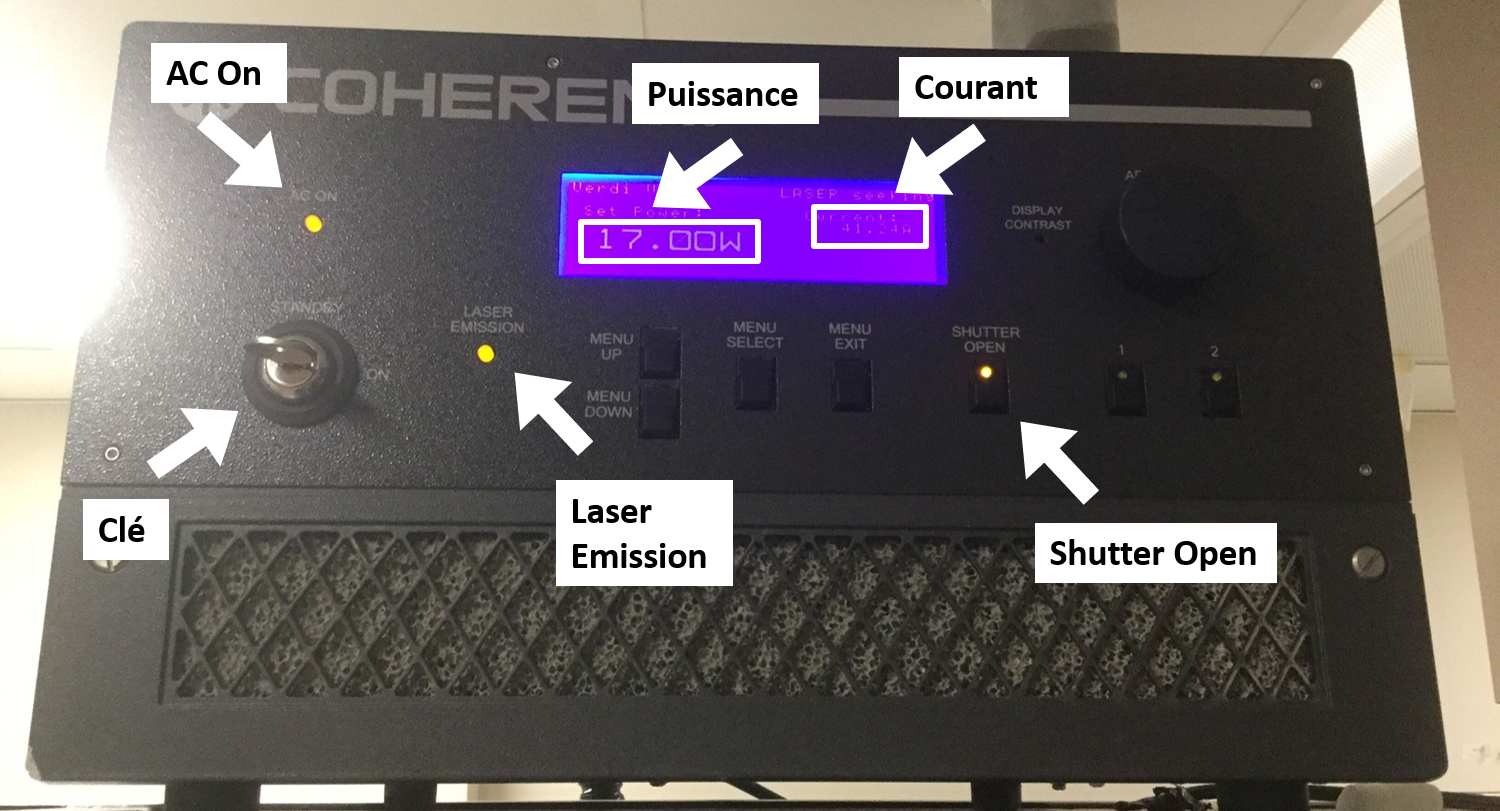
\includegraphics[width=12cm]{controleur-verdi.png}
        \caption{Contrôleur du \textit{Verdi}}
        \label{fig:controleur-verdi}
        \end{figure}
    \item Attendre que le laser se stabilise (environ 2-3 heures).
    \item Mettre des lunettes de sécurité: OD4 pour une longueur d'onde de 790~nm. 
    \\ Note: Le laser est pulsé et de puissance de plus de 1~W. Il est de classe 4.
    \item Vérifier que les deux refroidisseurs (voir figure~\ref{fig:cooler}) sont environ à 18-19$^\circ$C.
        \begin{figure}[H]
        \centering
        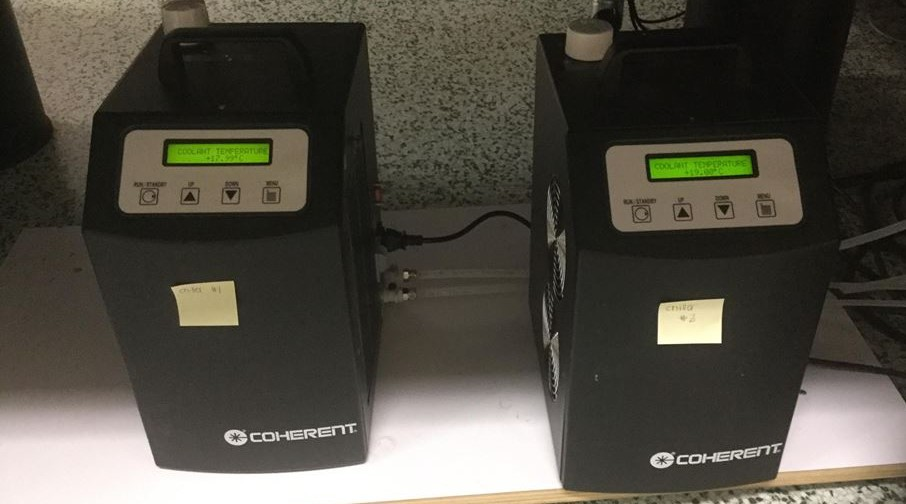
\includegraphics[width=10cm]{cooler.jpg}
        \caption{Refroidisseurs: l'un contrôle le \textit{Verdi}, l'autre le \textit{Mira} et le \textit{RegA}}
        \label{fig:cooler}
        \end{figure}
    Si non, remettre à la bonne température à l'aide des boutons \textit{flèches}. De plus, vérifier s'il y a de l'eau sur la table optique. Si oui, nettoyer le dégât d'eau et remplacer l'eau des refroidisseurs comme expliqué à l'Annexe~\ref{a:chillers}.
    \item Sur le \textit{contrôleur du Verdi} (voir figure~\ref{fig:controleur-verdi}), appuyer sur le bouton \textit{Shutter Open}.
    \item Vérifier que les lumières \textit{AC On}, \textit{Laser Emission} et \textit{Shutter Open} sont allumées.
    \item Vérifier que la \textit{puissance} est d'environ 17~W. Attendre que le \textit{courant} soit d'environ 44~A. Si ces conditions ne sont pas atteintes, remettre la clé sur \textit{Standby}, attendre 1 minute et recommencer à partir de l'étape \ref{etape1}.
\end{enumerate}